\documentclass[main.tex]{subfiles}
\begin{document}



\section{モデル}

プレイヤーが$N=\lbrace 内閣, 国会 \rbrace$の、2期間の不完備情報動学ゲームを考える。



司法を入れない理由は2つある。1つは、xxx。司法の違憲判決は行政執行や法律制定の数年から数十年に出される。
例として、旧優性法、足尾銅山。(TODO:他の例や、反対にすぐに政策が違憲/違法判定された例を調べる)。
その頃には、別の政権・議席割合であり、別のゲームをしていると考えるのが妥当。
2つ目は、見たかった司法の暴走の例は人質司法だが、これは政策決定とは別のゲームをしてる(司法の役割は、違法/違憲と合法/合憲の境目をはっきりさせる)。

主権者である国民(以下、"市民"とする)を入れない理由は、(TODO:結果は変わらないから国会に取り込んだ。)。


国会の効用関数を以下のように定義する。
$$u_\text{国会} = v_t(\;W\;,\; a_\text{国会}\;) × \delta^{t-1}_\text{市民}$$
$v_t(\;W\;,\; a_\text{国会}\;)$は、市民の厚生関数である。この厚生関数は、世界の状態である$W=\lbrace 有事, 平時\rbrace$と、国会が承認する政策$a_{国会}=\lbrace A, B\rbrace$によって決まる。
有事では投資的政策$A$が長期ではより効果的であり、平時では即時的政策$B$がより効果的であるとする。
時間割引率$\delta_{市民}=\lbrace \delta_L, \delta_H \rbrace (0\le \delta_L<\delta_H \le 1)$は、主権である市民が愚民($\delta_L$)であるか、賢民($\delta_H$)であるかを表している。
国会は、市民\footnote{モデル外}から直接声を聞くため、この市民の時間割引率$\delta_{市民}$を観測できるが、内閣は観測できない。

内閣の効用関数を以下のように定義する。
$$ u_\text{内閣} =\;\; \lbrace T\lbrace \alpha a_\text{国会} + \beta (1-a_\text{国会}) \rbrace  + (1-T)v_t(\;W\;,\; a_\text{国会}\;) \rbrace × \delta^{1-t}_{内閣}$$
内閣も市民の一人であるので、厚生関数$v_t(\;W\;,\; u_\text{国会}\;)$を同じように持つ。
加えて、内閣には私欲とも呼ばれる独自の正義感があり、各政策の実行自体からも効用を得る。それぞれ、投資的政策Aから得られる効用を$\alpha$, 即時的政策Bから得られる効用を$\beta$とする。
数式上では$a_{国会}=\lbrace A, B\rbrace = \lbrace 1,0\rbrace$とする。
この私欲と公共心の割合は$T:(1-T)$で表される。ただし、$T\in[0,1]$ 。
内閣は自身の私欲と公共心の割合$T:(1-T)$に加え、外交や調査機関の情報\footnote{これらはモデル外の話。}から世界の状態$W=\lbrace 有事, 平時\rbrace$を観測できるが、国会からは観測できないものとする。



\subsection{各権力の暴走の定義}
今分析の目的は、権力分立の機構が各権力の暴走をどのように防いでいるかを明らかにする、というものだ。そこで今モデル上での各権力の暴走をここで定義する。

まず、暴走の定義は「あるプレイヤーが市民の厚生関数$v_t(W, a_{国会})$の合計を最大化しようとしていない(TODO:見直す)状態」とする。
つまり、最適行動が市民の厚生関数$v_t(W, a_{国会})$の合計の最大化よりも重要なパラメータがある状態??
結果的には、市民の厚生関数$v_t(W, a_{国会})$の合計を最大化できる暴走もある。

内閣の暴走は、私欲にもとづく行政執行である。xxx

国会の暴走は、ポピュリズムである。xxx



\subsection{ゲームツリー}

\begin{figure}[htbp]
  \centering
  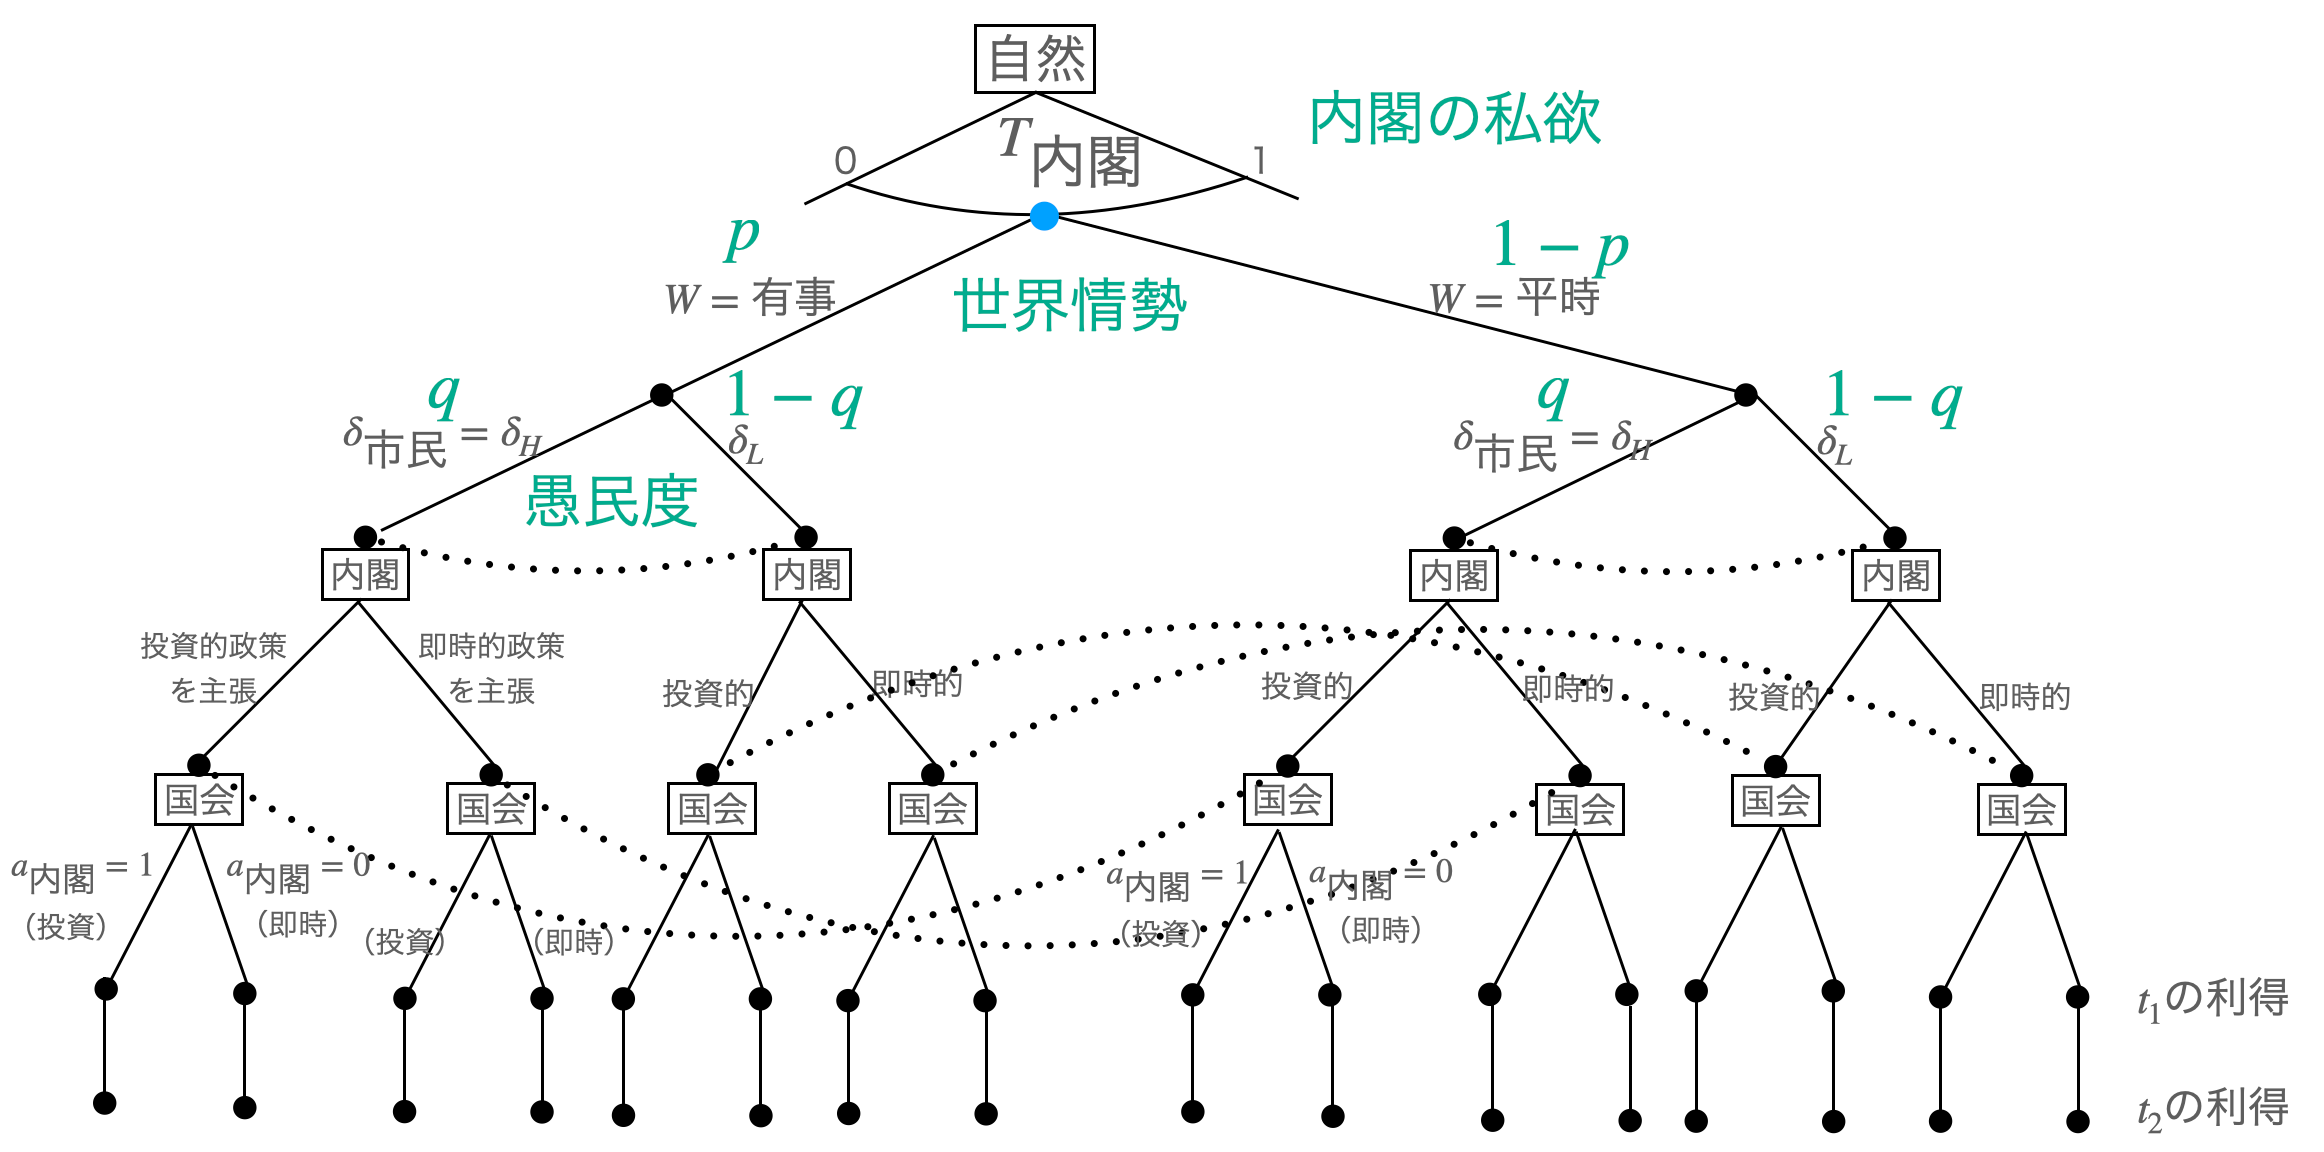
\includegraphics[width=0.7\textwidth]{./image/game_tree.png}
  \caption{ゲームツリー} 
  \label{fig:assumption_welfare_policy}
\end{figure}



ゲームは、自然が内閣と国会に私的情報を与えるところから始まる。まず自然は確率$p$で世界の状態を有事、$1-p$で平時とし、
内閣の私欲パラメーター$T\sim U(0,1)$\footnote{区間[0,1]の一様分布}を定める。これらの情報は内閣だけが観測することができる。
次に、自然は確率$q$で市民を賢民($\delta_{市民}=\delta_H$)とし、確率$1-q$で市民を愚民($\delta_{市民}=\delta_L$)とする。

内閣と国会の行動は全て1期で終わる。まず内閣は、どちらの政策が望ましいかというメッセージ$m_{内閣} = \lbrace A, B \rbrace$ を発する。
国会はそのメッセージを受けて、最終的にどちらの政策を承認するかを決定$a_{国会} = \lbrace A, B\rbrace$する。
直後、承認された政策が内閣により実行され、内閣と国会は1期目の利得を得る。

2期目は、どのプレイヤーも行動せず、実行された政策の2期目の利得を得る。




\subsection{市民の厚生関数$v_t(W, a_{国会})$における仮定}

\begin{figure}[htbp]
  \centering
  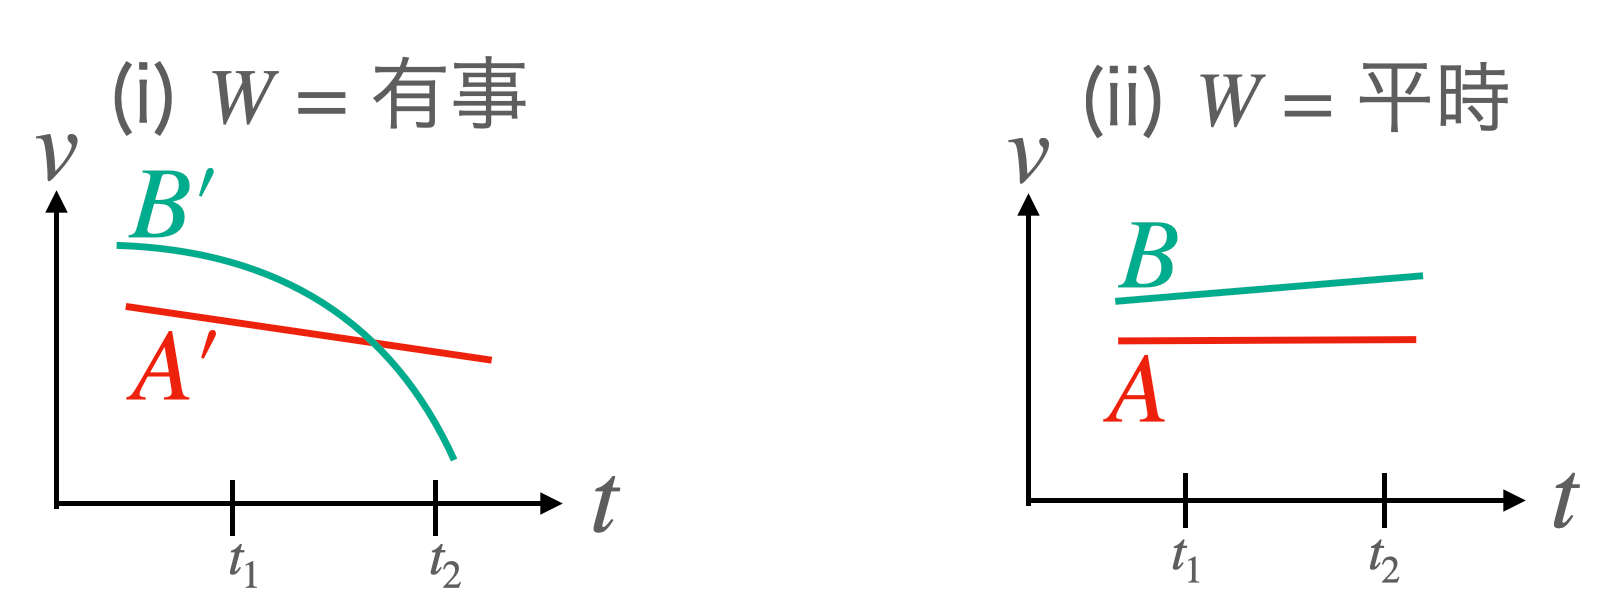
\includegraphics[width=0.7\textwidth]{./image/assumption_welfare_policy.png}
  \caption{厚生関数の仮定} 
  \label{fig:assumption_welfare_policy}
\end{figure}

有事における政策$A$によるt期の効用を$v'_{At}$とし、平時における政策$A$によるt期の効用を$v_{At}$とする。

世界の状態$W$が有事であっても平時であっても、即時的政策$B$の効用は変わらないものとする。
また前述の通り、有事では投資的政策$A$が長期的にはより効果的であり、平時では即時的政策$B$が長期的により効果的である。よって以下の仮定を得る。
\begin{assumption}  $v_{A1} + v_{A2}<v_{B1} + v_{B2} <  v_{A1} + v'_{A2}$ \end{assumption}


また、投資的政策$A$は実行に時間がかかるため、1期目における効用は平時でも有事でも変化がないが、2期目においてその効果が出るものとする。
さらに、平時または有事における各期の効用の大小関係、及び、平時と有事間での$A$政策の2期目の効用の差分と、$B$政策の1期目と2期目の差分の大小関係を以下のように仮定する。
\begin{assumption}  $v_{A1} < v_{B2} < v_{A2} < v_{B1} < v'_{A2}$  \end{assumption}
\begin{assumption}  $v_{A2} - v_{B1} < v'_{A2} - v_{B2}$\footnote{TODO:この過程は現実を反映したものではなく、計算上でxxxのため。}  \end{assumption}

上の図1はこれらの仮定を含めたものである。




\subsection{国会の時間割引率$\delta_{市民}$に関する仮定}

\begin{figure}[htbp]
  \centering
  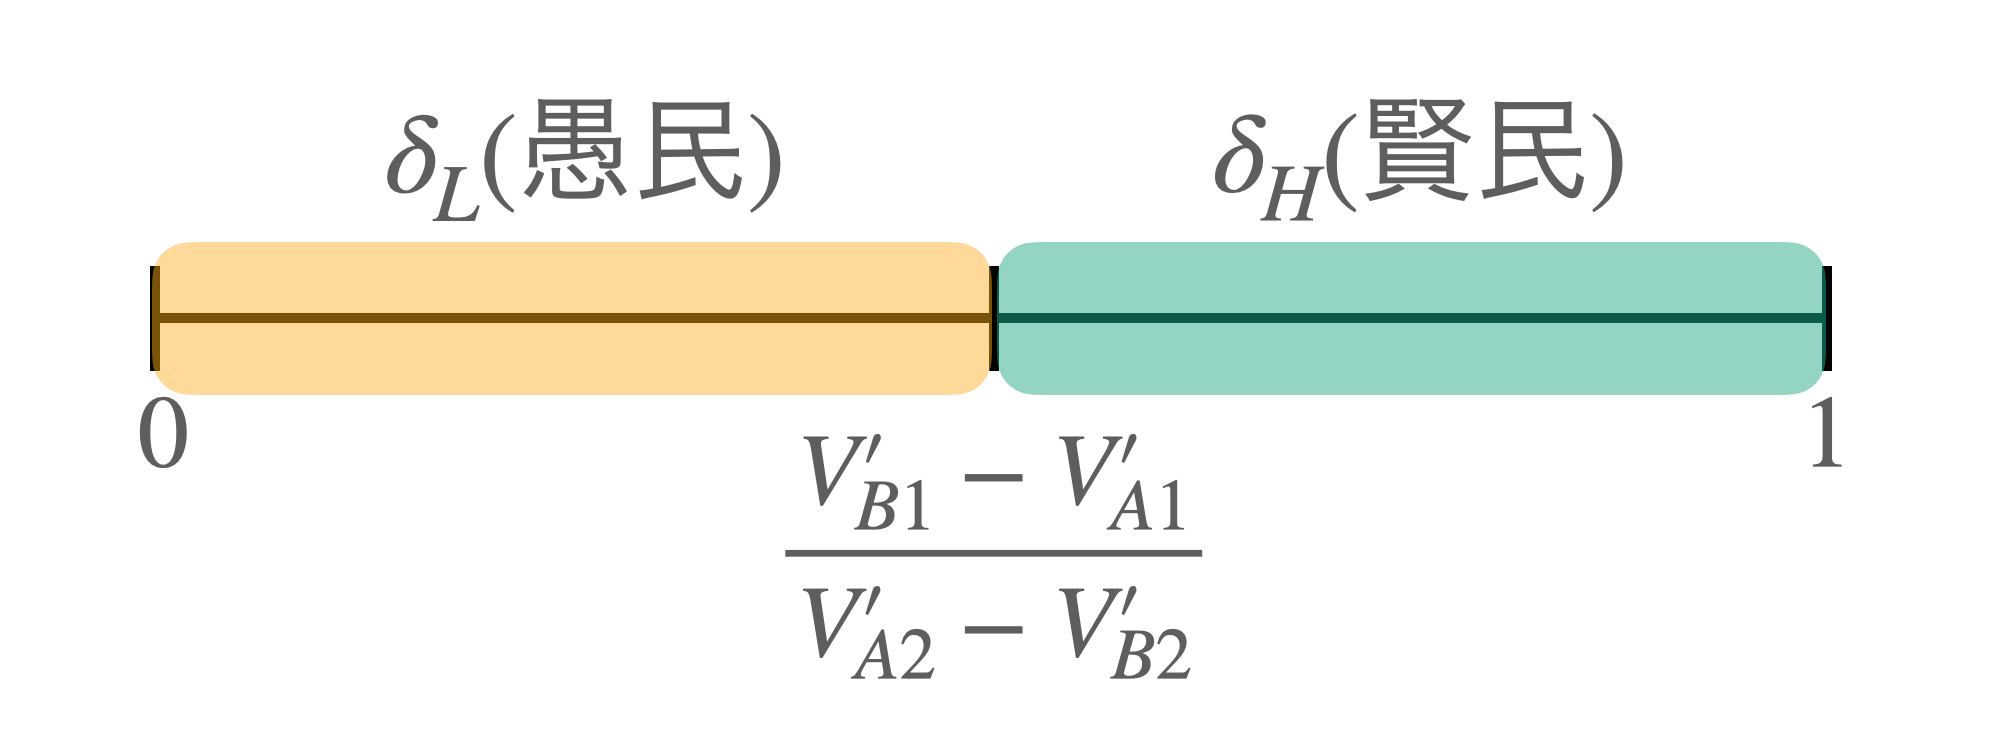
\includegraphics[width=0.7\textwidth]{./image/assumption_citizen_discount_rate.png}
  \caption{$\delta_{市民}=\lbrace \delta_L, \delta_H \rbrace$の仮定} 
  \label{fig:assumption_welfare_policy}
\end{figure}


前述の通り、$\delta_{市民}\in[0,1]$は主権者である市民が賢民($\delta_H$)か愚民($\delta_H$)かを表す。

賢民である場合は、有事では投資的政策、平時では即時的政策を望むものとする。これは例えば、社会保障が増大している時に増税を受け入れるような状態である。
数式上は$V_{B1} + \delta_H V_{B2} < V_{A1} + \delta_H V'_{A2}$ かつ $V_{A1} + \delta_H V_{A2} < V_{B1} + \delta_H V_{B2}$で表され、
整理すると$\frac{V_{B1} - V_{A1}}{V'_{A2} - V_{B2}} < \delta_H < \frac{V_{B1} - V_{A1}}{V_{A2} - V_{B2}}$となる。
これと$0 < \delta_H \le 1$を合わせて以下の仮定を得る。
\begin{assumption}  $\frac{V_{B1} - V_{A1}}{V'_{A2} - V_{B2}} < \delta_H \le 1$  \end{assumption}


愚民である場合は、平時であろうが有事であろうが即時的政策を望むものとする。これは例えば、給付金によるばら撒き政策を常に望む状態である。
数式上は$V_{A1} + \delta_L V'_{A2} < V_{B1} + \delta_L V_{B2}$かつ$V_{A1} + \delta_L V_{A2} < V_{B1} + \delta_L V_{B2}$で表され、
整理すると$ \delta_L < \frac{V_{B1} - V_{A1}}{V'_{A2} - V_{B2}} $となる。これと$0\le \delta_L < \delta_H$を合わせて以下の仮定を得る。
\begin{assumption}  $0 \le  \delta_L < \frac{V_{B1} - V_{A1}}{V'_{A2} - V_{B2}} $  \end{assumption}

上の図2はこれらの仮定を含めたものである\footnote{TODO:$\delta_{市民} = \frac{V_{B1} - V_{A1}}{V'_{A2} - V_{B2}}$の時は、考える意味がない or 愚民か賢民の方にくっつける。}。
つまり、$\frac{V_{B1} - V_{A1}}{V'_{A2} - V_{B2}}$を境として市民が賢民か愚民かが決まる。 






\theendnotes
\end{document}